\documentclass[12pt,oneside]{report}

%%% Load some useful packages:
%% "New" LaTeX2e graphics support.
\usepackage{graphicx}
%%	using final option to force graphics to be included even in draft mode
%\usepackage[final]{graphicx}
%% Tell graphicx the default directory for all figures
\graphicspath{{figures/}}

%% Enable subfigure support
\usepackage{subfigure}

%% Make subsubsections numbered and included in ToC
\setcounter{secnumdepth}{3}
\setcounter{tocdepth}{2}

%% Package to linebreak URLs in a sane manner.
\usepackage{url}

%% Define a new 'smallurl' style for the package that will use a smaller font.
\makeatletter
\def\url@smallurlstyle{%
  \@ifundefined{selectfont}{\def\UrlFont{\sf}}{\def\UrlFont{\small\ttfamily}}}
\makeatother
%% Now actually use the newly defined style.
\urlstyle{smallurl}

%% Define 'tinyurl' style for even smaller URLs (such as in tables)
\makeatletter
\def\url@tinyurlstyle{%
  \@ifundefined{selectfont}{\def\UrlFont{\sf}}{\def\UrlFont{\scriptsize\ttfamily}}}
\makeatother

%% Provides additional functionality for tabular environments
\usepackage{array}

%% Puts space after macros, unless followed by punctuation
\usepackage{xspace}

%% Make margins less ridiculous
\usepackage{fullpage}

%% Allows insertion of fixme notes for future work
\usepackage[footnote, nomargin]{fixme}

%%%% Turned off for tech report, should be turned on for research portfolio
%% Turn on double spacing
\usepackage{setspace}
\doublespacing

%% Make URLs clickable
%\usepackage[colorlinks, bookmarks=false]{hyperref}
\usepackage[colorlinks, bookmarks=true]{hyperref}

%% Since I'm using the LaTeX Makefile that uses dvips, I need this
%% package to make URLs break nicely
\usepackage{breakurl}

\usepackage{amsmath,amsfonts}
\numberwithin{equation}{subsection}
%%\usepackage{nonfloat}
\usepackage{bbm}
\usepackage{setspace}
\onehalfspacing
\usepackage{tabularx}

%%% End of preamble
\begin{document}

\title{Dissertation proposal: \\ [1.0cm]
       \textsc{Software Trajectory Analysis:} \\
       \textsc{An empirically based method for automated software process discovery} \\
       \author{Pavel Senin \\
							 Collaborative Software Development Laboratory \\
               Department of Information and Computer Sciences \\
               University of Hawaii \\[0.3cm]
               \texttt{senin@hawaii.edu} \\[0.3cm]
               CSDL Technical Report 09-09 \\
               \url{http://csdl.ics.hawaii.edu/techreports/09-09/09-09.pdf}
       }
       \date{August 2009}
}
\maketitle

\clearpage

%% Philip suggests it needs a ToC
\tableofcontents

%\begin{abstract}
%Abstract goes here if needed.
%\end{abstract}

%% Start with introduction
\chapter{Introduction}
Delivering high quality software products within the budget and in time is the main goal and the most 
challenging task of Software Engineering. Years of scientific research in this area resulted in a 
number of software processes providing detailed guidelines on how to reach 
the goal efficiently. These processes manifested themselfs as the means for improvements in terms 
of quality, speed and cost over existing practices. Many were implemented and tested within academic 
and industrial settings and proved proposed superiority. Some of these processes were successfully 
adopted and standardized in industry shaping the best practices of contemporary software development 
\cite{citeulike:9962021}. Moreover, there are plethora of processes for improving existing processes 
of software development on the team \cite{citeulike:9962027} and personal 
levels \cite{citeulike:9962022}.

The processes I am mentioning here are the well-known large formal models such as Waterfall and Spiral, 
as well as more flexible iterative agile approaches like XP, SCRUM or FDD. These are also sets of 
rules and recommendations which can be applied to certain stages of the software processes 
such as Test Driven Development or Pair Programming; there are general guidelines helping 
to improve the correctness of a product and standards, like CMMI or ISO 9000; guidlines for testing 
and measurements, code syntax rules and formatting styles, code comments 
recomendations \cite{citeulike:900855}. 

From the first sight, taking all this in account,  one would guess that 
the area of software processes is thoroughly explored and there are clear choices of processes 
and models for the one in charge making decision... But it is not true - despite many choices 
one can make, no one can foretell what is the ``best'' process to choose for certain constraints.
What managers are left with are the equal alternatives and vague promises. 
This deficiency in knowledge is the main coause of the ``software crisis'' phenomena point is supported by the fact that according to ``Chaos Report'' from the Standish 
Group (Rubinstein) \cite{SDTimes} only ``35\% of software projects in 2006 can be categorized as successful - meaning 
they were completed on time, on budget and met user requirements''. 
These thirty five percent of success clearly saying that it is somewhat difficult to make 
a statement that we are fully understand and able to control software processes. 
Moreover, over years, while this idea of a software process formalizations shaped the 
programming practices, which once thought to be a creative human activity accessible by amateurs 
and hobbyists \cite{citeulike:9958822} into a serious engineering discipline, bounded 
by requirements for education, standardized processes, rules, certifications, and strict 
financial requirements from stakeholders the opposite idea was born - the idea of 
software development as a craft. Interesting that such a duality of views can be found 
in the work of a single person \cite{citeulike:5203446}.

Clearly, there is a great room for research and improvement of our understanding of software processes.
This exploratory study is yet another attempt at the understanding. In my research work I am 
exploring techniques aiming the understanding of small processes which are 
rather the reflection of personal behaviors or habits of software development rather than a 
formalized constructs. Also, I would like to emphasize, that in this work I will not 
address the need and means of the process synthesis, its quality assessment, productiveness
or any topics related to the software product itself; I would rather focus on the specific issue - 
uncovering an existence and studying the programming habits. 

This thesis presents a methodology for finding recurrent behaviors through the 
analysis of the variety of software process artifacts left after performing a 
software process. I have called this methodology ``Software Trajectory'' and it consists 
of four distinct steps. Each of these steps has a specific goal and compromising variety of 
means to reach it. 
At first software process artifacts are identified and collected. 
At second, they are cleaned, organized and classified. 
On the third step particular research questions are formulated and data are organized and indexed. 
And finally, a set of KDD techniques is applied in order to undercover recurrent behaviors which 
could potentially shed a light on the performed process details. 

My personal motivation for performing this work is coming from the recognition of the 
importance of the software in our lives and the severity of issues with its development. 
Through my everyday experiences with software development and use I have stumble upon 
a number of issues which made me realize that mentioned ``software crisis'' phenomena is very real.
As a user in industrial and academic settings I often find myself facing software failures 
which create numerous difficulties for reaching production or research goals. As a developer, 
in an attempt to be productive and in order to deliver a better software I have studied and 
explored a number of formal processes, however, sometime I found myself seeing a very little of 
rationale behind their application, and moreover, in this exploration, when facing the process
application failing to help I was unable to comprehend what exactly went wrong and what need 
to be changed. All of these experiences made me studying software process research and exploring
novel approaches to software process recovery on my own in order to understand software process better.

\section{Research area overview}
As mentioned above, in this thesis I am focusing on a very narrow subject - exploring approaches
for uncovering of recurrent behaviors or ``programming habits'' out of software process artifacts.
Before narrowing further 


Software is usually coded by teams. Members of these teams are agreed and bound to use 
a particular technologies and development tools, they also agree on following well defined 
development process which is constrained by a timeline and budget. These are necessary 
constraints to keep work organized, however there is a great freedom in what they actually 
do in every single moment of time in order to progress towards lines of code which eventually 
will result in software. For example one developer may follow test first process while
another writes tests at last.  This freedom of choice in ordering of development activities 
while being much appreciated by talented and creative individuals creates an impression 
of chaotic and unordered activities for random observers, newbies and people in 
charge - so there we have all the attempts of imposing an order 
(or control) on all of the development activities. Metrics and models of processes






%% discuss some of related work
%%
\chapter{Related work} \label{related.work}
Although, process mining in the business domain is a well-established field with many work done and software developed up to date (ERP, WFM and other systems), the Business Process Intelligence tools usually do not allow to perform process discovery and typically offer relatively simple analyses that depend upon a correct a-priori process model \cite{citeulike:3718014} \cite{citeulike:5044991}. This fact restricts a direct application of the business domain process mining techniques to the general process mining and especially to the software engineering, where processes are usually performed concurrently by many agents, are more complex and typically have a higher level of noise. Taking this fact in account, I will review only some of the existing approaches to the general process mining which expressed possible applicability to the software process mining. 

Three papers are reviewed in this chapter: first one, by Cook \& Wolf \cite{citeulike:328044}, discusses an event-based framework for the process discovery based on the grammar inference and finite state machines. Authors directly applied their framework to the Software Configuration Management (SCM) logs demonstrating satisfiable results. Second paper, by van der Aalst et al \cite{citeulike:3718014}, demonstrates the applicability of the Transition Systems and labeled Petri nets to the process discovery in general. While authors are not inferring the direct application to the software process in this paper, the work by van der Aalst and Rubin \cite{citeulike:1885717} discusses this. The third paper by Jensen \& Scacchi while not presenting existing software or experimental validation describes an interesting and related framework of mining OSS repositories and archived communications aiming the process discovery. 

Other work has been done in the process mining and discovery which extends the reviewed papers in terms of dealing with concurrency. Among others, Weijters \& van der Aalst in \cite{citeulike:5128101} propose heuristics application to handle concurrency and noise issues, while van der Aalst et al in \cite{citeulike:5128101} discuss a genetic programming application.
\section{Process discovery through Grammar Inference} \label{grammar}
One of the most relevant to my research work done by Cook \& Wolf in \cite{citeulike:328044}. Authors developed techniques which they called \textit{``process discovery''}: they designed a framework which collects a software process data from ongoing process and generates a set of recurring patterns of behavior characterizing observed process. Under this work they augmented two methods of \textit{grammar inference} from previous work: neural network based and purely algorithmic method as well as developed their own Markovian method. The grammar inference can be defined as the process of infering a language grammar from the given set (sample) of sentences in the language. Once the grammar is inferred it could be converted into the (N)DFA which visualizes the observed phenomena. 

\begin{figure}[tbp]
   \centering
   \includegraphics[height=70mm]{inference.eps}
   \caption{Process discovery through the grammar inference: panel a) a sample event stream (simple process involving three types of events: Edit, Review, and Checkin); and FNA results obtained by applying three methods of process discovery from Cook \& Wolf \cite{citeulike:328044}.}
   \label{fig:inference}
\end{figure}

The first method, neural network based grammar inference method RNet, adopted by authors defines a recurrent neural network architechture which characterizes current system state looking on the past behavior. Once the neural net is trained, authors extract the FSM by presenting different strings to the net and extracting the hidden neurons activity through observations. By the nature of Neural Net, the closely related activation patterns clustered into the same state. By noting the current pattern, the input token, and the next activation pattern transitions are recorded and compiled into inferred FSM later.

The second approach taken, a purely algorithmic KTail method, augmented by authors from Biermann \& Feldman \cite{citeulike:5120603}. The idea is that a state is defined by what future behaviors can
occur from it. The \textit{future} is defned as the set of next $k$ tokens. Obviously, two or more strings can share a common prefix and then diverge from each other providing features for building a corresponding FSM.

The Markov based method developed by authros is taking in account past and future system behavior in order to guess the current system state. Assuming that a finite number of states can defined the process, and that the probability of the next state is based only on the current state (Markov property) authors build a $n^{th}$-order Markov model using the first and second order probabilities only. Once built, the probability table corresponding to the markov model converted into FSM which further reduced basing on the user specified cut-off threshold for probabilities.

Authors implemented all discussed algorithms in a software tool called DaGama as a plugin for larger software system Balboa \cite{citeulike:5120757}. 

Overall, while having some issues with the complexity of produced output and noise handling, authors proved applicability of implemented algorithms to the real-world process data by demonstrating an abstraction of the actual process executions and capturing important properties of the process behavior. Major backdraw of the approach as stated by authors lies in the inability of the FSMs to model concurrency of processes whether the software development process is usually performed by the many agents simultaneously.
\section{Incremental Workflow Mining with Petri Nets}
Another set of findings relevant to my research approach was developed by Rubin et al. \cite{citeulike:1885717} and van der Aalst et al \cite{citeulike:3718014} and is called \textit{incremental workflow mining}. The authors not only designed sophisticated algorithms but built a software system using a business process mining framework called ProM by van Dongen et al. \cite{citeulike:5043673} which synthesizes a Petri Net corresponding to the observed process. The system was tested on SCM logs and while the process artifacts retrieved from the SCM system are rather high-level, the approach discussed is very promising for the modeling of software processes from the low-level product and process data.

\begin{figure}[tbp]
   \centering
   \includegraphics[height=65mm]{petri.eps}
   \caption{Illustration of the ``Generation and Synthesis Approach'' from \cite{citeulike:5043673}: a) Transition System with regions shown; b),c) Petri Nets synthesized from the Transition System.}
   \label{fig:petri}
\end{figure}

Within the incremental workflow mining framework, the input data from the SCM audit trail information is mapped to the event chain which corresponds to the software process artifacts. The authors call this process \textit{abstraction on the log level} which is implemented as a set of filters which not only aggregates basic events into single high-level entities but also removes data irrelevant to the mining process (noise). 

The event chain constructed through the abstraction is then treated with the \textit{Generate} part of the \textit{``Generate and Synthesis''} \cite{citeulike:3718014} algorithm in order to generate a \textit{Transition System} which represents an ordered series of events. This algorithm looks at the history (prefix) and the future (suffix) sequences of events related to the current one in order to discover transitions.  When applied to the abstracted log information, the algorithm generates a rather large Transition System graph where edges connect to abstracted events. This transition system is then successively simplified by using various reduction strategies such as ``Kill Loops'', ``Extend'', ``Merge by Output'' and others; it is possible to combine these reduction strategies in order to achieve a greater simplification.

At the last step of the incremental workflow mining approach, Transition Systems are used to \textit{Synthesize} labeled Petri nets (where different transition can refer to the same event) with the help of \textit{``regions theory''} \cite{citeulike:5128170}. As with the Transition System generation, the authors investigate many different strategies of Petri nets synthesis, showing significant variability in the results achieved. (see Figure \ref{fig:petri}).

The significant contribution of this research is in the generality of the method. It was shown that by tuning the ``Generate'' and ``Synthesize'' phases it is possible to tailor the algorithm to a wide variety of processes. In particular, as mentioned before, Rubin et al. successfully applied this framework to the SCM logs analysis.

%% review implemented and tested methods
%%
\chapter{Methods}

\section{Symbolic Aggregate approXimation (SAX)}

\section{Multivariate extension of SAX}

\section{Indexing}
\section{Piecewise Approximation of time-series (PLA, PCA, PAA, APCA)}
Following the first wave of time-series similarity methods based on the spectral decomposition such as DFT, DCT, SVD, CHEB\footnote{Chebyshev polynomials based decomposition methods were omitted in this review due to the space constraints and could be found in \cite{citeulike:2753031} and overall very similar to APCA in performance}
and Haar wavelets, another approach has become popular among the time-series data-mining community: piecewise approximation. Faloutsos et al \cite{citeulike:4344279} proposed Piecewise Flat Approximation, Morinaka et al \cite{citeulike:4295248} and Chen et al \cite{citeulike:4165220} proposed Piecewise Linear Approximation (PLA), Yi \& Faloutsos \cite{citeulike:2946589} and Keogh et al \cite{citeulike:3000416} followed with Piecewise Aggregate Approximation (PAA), Chakrabarti et al \cite{citeulike:1736140} proposed Adaptive Piecewise Linear Approximation (APLA). All this work has shown that surprisingly simple piecewise-based approximation methods outperform previous spectral decomposition based techniques by being easy to compute and index while satisfying the contractive property condition (\ref{eq:bounding}).

We will review the PAA method which approximates the time-series $X$ of length $n$ into vector $\bar{X} = ( \bar{x}_{1}, ..., \bar{x}_{M} )$ of any arbitrary length $M \leq n$ where each of $\bar{x_{i}}$ is calculated by following the next formula:
\begin{equation}
\bar{x}_{i} = \frac{M}{n} \sum_{j=n/M(i-1)+1}^{(n/M)i} x_{j}
\label{eq:paa}
\end{equation}

This simply means that in order to reduce the dimensionality from $n$ to $M$, we first divide the original time-series into $M$ equally sized frames and secondly compute the mean values for each frame. The sequence assembled from the mean values is the PAA transform of the original time-series. It was shown by Keogh et al that the complexity of the PAA transform can be reduced from $O(NM)$ (\ref{eq:paa}) to $O(Mm)$ where $m$ is the number of sliding windows (frames). The satisfaction of the transform to bounding condition in order to guarantee no false dismissals was also shown by Yi \& Faloutsos and Keogh et al by introducing the distance:
\begin{equation}
D_{PAA}(\bar{X}, \bar{Y}) \equiv \sqrt{\frac{n}{M}} \sqrt{ \sum_{i=1}^{M} 
\left(  \bar{x}_{i} - \bar{y}_{i} \right)}
\label{eq:paa_distnace}
\end{equation}
and showing that $D_{PAA}(\bar{X}, \bar{Y}) \leq D(X,Y)$.

Concluding the piecewise based time-series approximation methods review we should note that PAA is very similar to Haar-wavelet based approach \cite{citeulike:4384535} as shown at Figure \ref{fig:paa_comparison}. Another nice feature of the PAA is the ability to process range queries with sequences of unequal to index size dimension, as was shown by Keogh et al in \cite{citeulike:3000416}.
\begin{figure}[tbp]
   \centering
   \includegraphics[height=95mm]{paa_comparison.eps}
   %%{seriesheatmap}
   \caption{The combination of figures from \cite{citeulike:3000416} depicts different approaches for the time-series approximation (decomposition): a) the time-series spectral approximation (Fourier); b) SVD-based approximation; c) Haar-wavelet based approximation; d) Piecewise Aggregate Approximation where transformed values shown as ``box'' basis functions.}
   \label{fig:paa_comparison}
\end{figure} 

Overall, the PAA based approach to the time-series similarity problem was found to be very competitive in precision to the spectral-decomposition based methods while outperforming all competitors in the speed of index building. In terms of the index performance, PAA index has a constant time of insertions and deletion whether in case of SVD, for example, we have to rebuild the whole matrix. Also, Keogh et al has shown that PAA has ability to handle weighted Euclidean distance metrics, allowing implementation of more sophisticated querying techniques like ``relevance feedback'' \cite{citeulike:4406444}.

\section{Symbolic Aggregate approXimation (SAX)}
The last approach for the time-series similarity problem we are reviewing in this writing is the current state of the art time-series representation and dimensionality reduction method called Symbolic Aggregate approXimation (SAX) which transforms original time-series data into symbolic strings. This method, proposed by Lin et al \cite{citeulike:2821475}, turns out to be not only extremely simple and computationally cheap, but also fast and precise in the range-query processing. Moreover, the use of the symbolic representation opens door to the existing wealth of data-structures and string-manipulation algorithms in computer science such as hashing, suffix trees, regular expression pattern matching, etc.

SAX transforms a time-series $X$ of length $n$ into the string of arbitrary length $\omega$ where typically $\omega << n$, using an alphabet $A$ of size $ a \geq 2$. The SAX algorithm consist of two steps: at the first step it transforms the original time-series into PAA representation and this intermediate representation than converted into the string during the second step. Use of the PAA at the first step brings an advantage of simple and efficient dimensionality reduction while providing the important lower bounding property. Second step, actual conversion of PAA coefficients into letters also computationally efficient and the lower bounding of symbolic distance was proven by Lin et al.

Discretization of the PAA representation of the time-series into SAX implemented in a way which produces symbols corresponding to the time-series features with equal probability. The rigorous analysis of the time-series datasets available for authors shows that normalized by the zero mean and unit of energy time-series follow the Normal distribution law. By using the Gaussian distribution properties \cite{citeulike:167581} it's easy to pick $a$ equal-sized areas under the Normal curve. The points of the cut lines slicing the the under-the-Gaussian-curve area called ``breakpoints''.
\begin{figure}[tbp]
   \centering
   \includegraphics[height=45mm]{sax_intro.eps}
   \caption{The illustration of the SAX approach taken from \cite{citeulike:2821475} depicts two pre-determined breakpoints for the three-symbols alphabet and the conversion of the time-series of length $n=128$ into PAA representation first and following mapping of the PAA coefficients into SAX symbols with $w=8$ and $a=3$ resulting in the string \textbf{baabccbc}.}
   \label{fig:sax_intro}
\end{figure}

Extending Euclidean \ref{eq:euclidean_distance} and PAA \ref{eq:paa_distnace} distances, the function returning the minimal distance between two string representations of original time series $\hat{Q}$ and $\hat{C}$ defined as
\begin{equation}
MINDIST(\hat{Q},\hat{C}) \equiv \sqrt{ \frac{n}{w} } \sqrt{ \sum_{i=1}^{w} ( dist( \hat{q}_{i}, \hat{c}_{i} ) )^{2}}
\label{eq:sax_mindist}
\end{equation} 
where the $dist$ function is implemented by using the lookup table for the particular set of the breakpoints as shown in table \ref{tbl:sax_lookup} where the singular value for each cell $(r,c)$ is computed as 
\begin{equation}
cell_{(r,c)} = 
\begin{cases} 
0, \text{ if }\left| r-c \right| \leq 1 \\
\beta_{\max(r,c) - 1} - \beta_{\min(r,c) - 1}, \text{ otherwise}
\end{cases}
\label{eq:cell}
\end{equation}
\begin{table}
\begin{tabularx}{400pt}{X X X X X}
\hline
   & a   & b    & c    & d    \\
\hline
a & 0    & 0    & 0.67 & 1.34 \\
b & 0    & 0    & 0    & 0.67 \\
c & 0.67 & 0    & 0    & 0    \\
d & 1.34 & 0.67 & 0    & 0    \\
\hline
\end{tabularx}
\caption{A lookup table used by the MINDIST function for the $a=4$}
\label{tbl:sax_lookup}
\end{table}
\begin{figure}[tbp]
   \centering
   \includegraphics[height=47mm]{sax_distance.eps}
   \caption{The visual representation of the two time-series $Q$ and $C$ and three distances between their representation: Euclidean distance between raw time-series (A), the distance defined for PAA coefficients (B) and the distance between two SAX representations (C).}
   \label{fig:sax_distance}
\end{figure}


As shown by Li et al, the introduced SAX distance measure lower-bounds the PAA distance, i.e.
\begin{equation}
\sum_{i=1}^{n} (q_{i} - c_{i})^{2} \geq n(\bar{Q} - \bar{C})^{2} \geq n(dist(\hat{Q},\hat{C}))^2
\label{eq:sax_bounding}
\end{equation}

\section{Temporal models, concepts and operators} \label{tconcepts}
The SAX transformation procedure described in the previous section yields symbolic time-series based on the real-valued data. Having such a symbolic representation, also called in the literature as \textit{symbolic temporal data}, is very adventageous comparing to the real-valued data in terms of easy pattern search, indexing, clustering and low computational and space complexity. 

This section built around the technical report by Fabian M\"orchen \cite{citeulike:1748833} which aggregated many of work done in the field of data mining from symbolic temporal data. Two figures taken from this work constitute the Figure \ref{fig:concepts1} and depict a hierarchy of time-points (left panel) and time-intervals (right panel) data models, concepts and operators.

\begin{figure}[tbp]
   \centering
   \includegraphics[height=45mm]{concepts1.eps}
   \caption{The temporal concepts and operators from \cite{citeulike:1748833} for both: time point and time interval data models.}
   \label{fig:concepts1}
\end{figure}

\subsection{Temporal data models} \label{tconcepts_models}
The time intervals temporal data model built upon the concept of \textit{duration} which is a repetition of the property over several time-points. More precisely, \textit{time-intervals} are continous groups of discrete time instants and some algorithms and applications operate with them rather than individual points. Time-intervals essentially are sets of two or more continous points and two successive time points define a minimal interval which starts at the earlier point and continues to the latter point inclusevily. Allen \cite{citeulike:191348} says: ``In English, we can refer times as points or as intervals...'' giving next two examples: ``We found the letter at twelve noon.'' and ``We found the letter while John was away.'' pointing that there are temporal relations involved.

\subsection{Temporal concepts} \label{tconcepts_concepts}
The concept of \textit{concurrency} as described by the author explains the closeness of two time-points in time without considering their ordering, - a coincidence of events in time is important. The \textit{synchronicity} is a special case of concurrency where events occur synchonously in time.

The \textit{order}, and \textit{synchronicity} concepts in the Time intervals model are anlogous ones in the Time points model, whether the Time intervals \textit{coincidence} describes an intersection of intervals in time.

\subsection{Temporal operators} \label{tconcepts_opertaors}
The time point operators from the Figure \ref{fig:concepts1}: \textit{before}, \textit{after} and \textit{equals} precizely define the relation of points in time. The \textit{close} operator is a ``fuzzy extension for temporal reasoning'' since it encapsulates other three. Note that some threshold can be used to relax or constrain these operators, for example we can consider points equal to each other even if they are less than $k$ time units apart.

The Time intervals operators a more complex and were examined in many mork. In 1983 Allen \cite{citeulike:191348} proposed therteen basic relations between time intervals which are distinct, exhausting and qualitative. In his work Allen showed that thirteen relationships are sufficient to model the relationship between any two intervals. Figure \ref{fig:allen} depicts Allen's relations. This relations and operations on them are forming \textit{Allen's Interval Algebra}.

Despite the exhausting property of Allen's relations, while working on the multimedia data analysis, Snoek \& Worring \cite{citeulike:272197} discovered two practical problems: first is that ``in video analysis, exact alignment of start- or end- points seldom occurs due to noise... '' and the second is that ``two time intervals will always have a relation even if they are far apart in time...''. In order to resolve these issues authors had to relax a set of Allen's relations and introduce a new \textit{NoRelation} relation. This new relaxed set of 14 relations named TIME (Time Interval Multimedia Event) was built with two time-interval parameters: $T_{1}$ for the neighborhood in which impresize boundary segments considered synchronous and $T_{2}$ which assigns two intervals as \textit{NoRelation} if they are more than $T_{2}$ time apart.

citeulike:4991332

\begin{figure}[tbp]
   \centering
   \includegraphics[height=20mm]{allen.eps}
   \caption{The Allen's thirteen basic relations (from \cite{citeulike:4072008}) sorted by the degree to which $a$ begins and later ends before $b$. All but \textit{equals} can be inverted.}
   \label{fig:allen}
\end{figure}

\section{Temporal patterns and indexing} \label{tpatterns}
In previous sections of this chapter we have shown the SAX algorithm for conversion of real value time series into symbolic representation along with introducing temporal data models, concepts and operators. All these was a necessery bakground in order to continue with approaches taken for unsupervised pattern mining from symbolic temporal data. In this section we will review sequential pattern mining algorithms from time points for univariate and multivariate data along with mining algorithms for time interval data.

Before discussing algorithms we need to define patterns of interest we are looking for. For many data mining areas such as such as medicine, motion-capture, robotics, video surveillance, meteorology and others detection of \textit{repeated} or \textit{approximately repeated} patterns plays essential role. These repeated patterns are named as \textit{motifs}. From other hands, in the same and other ares detection of the unusual (novelty) patterns has the same or even greater value, for example unusual semi-repeated noize in the ECG data or unusual activity patterns in video surveillance. These patterns, which appear uniquely or with some frequency highly different from expected, named as \textit{surprise patterns}.


\subsection{Time points patterns}
According to M\"orchen, the most commonly searched pattern within univariate symbolic time series is order. This search for particular order of symbols within subsequence is not necesserely requires symbols to be consecutive, usually gaps and substitution allowed. The very similar problem of string matching is one of the central in the computation biology \cite{citeulike:465665} and many algorithms are very similar. The suffix tree algorithm is a standard approach for pattern discovery from the string time-series according to Palopoli et al \cite{citeulike:5003338}. Authors discussing algorithms of automatic discovery of frequent structured patterns (\textit{motifs}) in ``exact'' or ``approximate'' forms. 

As an opposite to motif finding problem, a \textit{surprise pattern} problem explored too. In many fields: biology, physics, astronomy and statistics various algorithms proposed. Keogh et al in \cite{citeulike:3025877} discuss methods of finding a surprise patterns from the temporal data and propose their ``TARZAN'' algorithm which is reporting surprising patterns occuring with substantially different frequency from that expected by chance.

%% talk about the implementation
%%
\chapter{Hackystat-Trajectory - software process mining framework.}
the implementation of a system aiding in discovery of novel software process knowledge (shown at the Figure \ref{fig:system_overview});

\section{Framework overview.}

\section{Framework architecture.}

\section{Database schema design.}

%% discuss experiments
%%
\section{Planned evaluation in the classroom}
Aiming a discovery of novel recurrent behavioral patterns in the software process, I am planning to conduct a classroom case study. The approach I am taking is based on the daily re-indexing and mining of the software process data collected by Hackystat from the classroom software project development during the Fall'09 and Spring'10 Software Engineering classes along with interaction with students. 

After collecting a certain amount of data, I expect to see some recurrent patterns gaining enough support to be considered as ``candidate patterns''. The function I am considering as support, will be a product of two metrics: one is based on the support function from AprioriAll algorithm and quantifies the fraction of the developers demonstrating the same pattern, and the second one is based on the total frequency of pattern appearance. The pool of these candidate patterns will be built and reviewed on the daily basis. By reviewing candidate patterns, I am planning to fulfill two goals: first is to identify truly useful and interesting patterns, and second is to enhance a knowledge base of the data-mining algorithm limiting the amount of reported unmeaningful or trivial patterns. The ability to capture patterns and communicate with students in real-time will be extremely helpful in this process providing mechanism for validation of my own guesses.


\section{Planned evaluation using public data}
In addition to the classroom experiments, I am planning to evaluate my research through the use of publicly available repositories. This validation is aiming to assess the ability of my approach to reproduce already published results indicating correctness and similar to other tools performance. If I can find some novel patterns within this data, it will provide a second form of evidence for the utility of my research.

As the main source of the data for the validation, I am planning to use public SCM repositories whose mining is traditionally used in the ``MSR Challenges'' \cite{citeulike:5043676} and published in proceedings of ``IEEE International Conference on Mining Software Repositories''. Following this popular approach, I will try to apply my framework to SCM repository artifacts with the goal of reproducing some of the published results and ultimately participating in the challenge. Second, there are various public data hosted by the ``PROMISE software engineering repository'' \cite{Sayyad:2005} which contains two kinds of data: the software product datasets used for the building of the predictive software models, and some ``universal'' data sets representing SACM repository transaction. Most of these datasets were used for a number of publications and I am planning to evaluate my framework by attempting to reproduce these results. 
\section{Pilot study}

\section{Planned evaluation in the classroom}

\section{Planned evaluation using public data}



%% anticipated contribution
%%
\chapter{Anticipated contribution} \label{contribution}

%%% Input file for bibliography
\bibliography{seninp}
%% Use this for an alphabetically organized bibliography
\bibliographystyle{plain}
%% Use this for a reference order organized bibliography
%\bibliographystyle{unsrt}
%% Try using this BibTeX style that hopefully will print annotations in
%% the bibliography. This will allow me to make notes on papers in the
%% BibTeX file and have them readable in the references section until
%% I turn them into a conceptual literature review 
%\bibliographystyle{annotation}

\chapter{Appendices} \label{appendix}

\section{Interview procedure}
I plan to conduct two offline interview sessions empirically evaluating both: the performance of the Trajectory framework and the usfullness of discovered patterns. The interview format during my work on the TrBy the beginning of the Fall'09 semester, I plan to design a taxonomy and implement a low-level software process events abstraction into symbolic representation. The database schema will be extended for storing these data and indexes. Immediately after that, I will proceed with the implementation of fundamental algorithms for associated and sequential patterns mining. This new data model and KDD toolkit will allow me to discover more low-level behavior patterns some of which might be found useful though the empirical evaluation during the period of data collection from the Fall'09 Software engineering class. I will be working with those students who will demonstrate a relevant recurrent behavior in software process for clarification of observed phenomena.

\newpage


\end{document}